\newcommand{\ov}[1]{\overline{#1}}
\newfloat{Example}{thp}{loe}[section]
\newcommand{\unaryminus}{\scalebox{0.5}[1.0]{\( - \)}}
\newcommand{\AND}{\texttt{AND}\xspace}
\newcommand{\RST}{\texttt{RST}\xspace}
\newcommand{\CLK}{\texttt{CLK}\xspace}
\newcommand{\HOLDN}{\texttt{HOLDN}\xspace}
\newcommand{\MULI}{\texttt{MULI}\xspace}
\newcommand{\MULO}{\texttt{MULO}\xspace}
\newcommand{\infer}{\texttt{infer}\xspace}
\newcommand{\multype}{\texttt{multype}\xspace}
\newcommand{\pipe}{\texttt{pipe}\xspace}
\newcommand{\mac}{\texttt{mac}\xspace}
\newcommand{\ready}{\texttt{ready}\xspace}
\newcommand{\start}{\texttt{start}\xspace}
\newcommand{\holdn}{\texttt{holdn}\xspace}
\newcommand{\nready}{\texttt{nready}\xspace}
\newcommand{\STDV}{\texttt{STD\_LOGIC\_VECTOR}\xspace}



\section{Improved Arithmetic Cores}
\label{sec:arth}

This section will explain the design process for the multiplier and divider units.
For each the rationale behind the chosen scheme will be detailed, along with its principal advantages and disadvantages.
This analysis will necessarily feature a comparison between the different possibilities considered.

Thereafter details of the implementation will be given along with the important handshaking signals that ensure the interface between the units and the processor. Finally, the verification phase will be presented. This includes the testbenches used during the development processed.

As previously stated, in order to improve the performance of the arithmetic unit we redesigned from the ground up both the
two units: multiplier and divider.

Alternatively the original multiplier can be configured for 2 or 4 cycles of latency (instead of 5) through the use of \texttt{make xconfig}.
So although we are writing a new unit it is necessary to configure the
processor with the appropriate latency as well, so it can handle the
handshaking signals generated by our multiplier in the correct way.

For the divider there is not a previous configuration, so the processor knows that an operation is
completed by inspecting the \texttt{ready} and \texttt{nready} signals which have been reproduced following the
specifications.

The part of the core that handles the other signals such as \texttt{start}, \texttt{flush} or \texttt{holdn}, has been designed
to mimic the original version, thereafter all the handshaking signals are handled and generated following the
specifications to enable unit compatibility with the processor.
A more detailed description of these interface signals is presented later in sections~\ref{sec:mul} and \ref{sec:div}, respectively for the multiplier and for the divider.


\subsection{Multiplier}
\label{sec:mul}

The simplest multiplier consists of an iterative shift-add routine, which works, as the name implies, adding pairs of bits, accumulating the result and shifting it appropriately. This closely resembles the pen-and-paper algorithm for multiplication. The main hindrance of this technique is the serial nature. It is necessary to wait for one result to advance to the next operation. Therefore a \texttt{n-bit$\times$m-bit} operating costs $n+m$ cycles. On the other hand is very compact and uses very few components, so the power consumption is low. Nonetheless due to its latency it is not suitable for this project.

Another easy solution would be to define a look-up table multiplier. For this, all possible combination of inputs are tested and the corresponding results are stored for later retrieval. This makes the multiplier very fast but the table size grows exponentially. Therefore for our input sizes this option is not suitable.

In order to improve the performance there are two possibilities:
\begin{itemize}
\item Reduce the number of operands (\ie high-radix multipliers)
\item Adding the operands faster (\ie tree and array multipliers)
\end{itemize}

Starting with the first item, high-radix operations have several advantages.
They can reduce the size of the operands by ``compressing'' them in a higher radix.

First, the original operands are converted to the new radix. Then the necessary computations are performed on the converted values. And finally the result is converted back to the original representation.

The translation steps add some overhead to the process and therefore the number of operations on the converted values should be large enough to marginalize the introduced overhead.

Handling ``dificult'' multiples, such as 3, is also an issue. A possible solution is precomputing these values or rewriting them, \eg $3a = 4a - a$. However these solutions for the corner cases add some complexity and irregularity to the circuit.

Booth recoding is another way to improve the first method. To recode the operand we replace the LSB of a series of 1s by -1 and the first 0 after that series by 1. Thereafter we group each pair and add the result (in radix 4). Example~\ref{ex:booth} from~\cite{book} demonstrates this procedure.

\begin{center}
\captionsetup{type=table}
$\begin{array}{ccccccccl}
10  & 01 & 11  & 01 & 10 & 10 & 11 & 10 & \quad\text{Operand } x\\
\unaryminus10 & 10 & 0\unaryminus1 & 10 & \unaryminus11 & \unaryminus11 & 00 & \unaryminus10 &\quad \text{Recoded Version } y\\
\midrule
\unaryminus2 & 2 & \unaryminus1 & 2 & \unaryminus1 & \unaryminus1 & 0 & \unaryminus2 & \quad\text{Radix-4 Version } z\\ 
\end{array}$
\captionof{Example}{Example for radix-4 Both recoding (originally from~\cite{book}).}
\label{ex:booth}
\end{center}

The main advantage is halving the number of partial products while keeping the circuit simple (there are no \emph{difficult} multiples).
Booth recoding can be combined with Carry Save Adders for fast multiplication. Actually this combination results in a well balanced solution in the \emph{Multiplier Design Spectrum}. It ranges from simple but slow multipliers to very fast but expensive choices (\ie Full tree).
However since performance is out first class design constraint it was decided to use a Wallace Tree which is a variation in CSA tree design. The respective details and consequent implementation are featured in section~\ref{sec:wallace}.

\subsubsection{Wallace Tree Multiplier}
\label{sec:wallace}

For this project it was decided the most appropriate multiplier scheme would be the Wallace Tree Multiplier. The most important reason for this choice is due to its great performance although at the cost of gates and area.
The Wallace tree is a regular hardware structure to multiply two operands. It was invented by Chris Wallace, an Australian Computer Scientist in 1964.

The algorithm can be divided in three major steps:
\begin{enumerate}
\item The initial \AND operation between all combinations of bits of each operand. The weights must be adjusted according to the location of the operands, just like in the well known pen-and-paper algorithm. The resulting tree, using dot notation, is shown in figure~\ref{fig:wallace_tree}.

\begin{figure}[H]
\centering
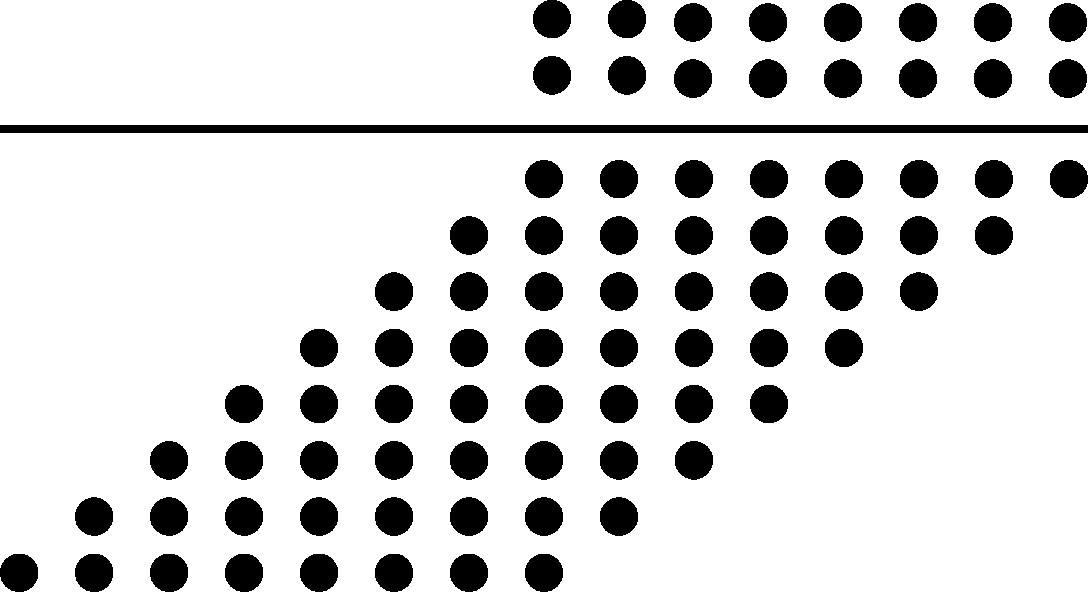
\includegraphics[width=0.70\textwidth,height=0.4\textheight,keepaspectratio]{Wallace_tree_8x8_trimmed.pdf}
\caption{Resulting tree after executing step 1 for and 8 bit by 8 bit multiplication.}
\label{fig:wallace_tree}
\end{figure}

\item Thereafter the tree must be reduced through the use of half adders and full adders. These will convert each two or three ``dots'', respectively, into one and a carry out for the following column. This step shall be iterated sufficient times until only two numbers emerge.

\item Finally, the two remaining numbers can be summed with a conventional adder. The width of the result should be equal to the sum of the widths of the original operators. For example for a 32 bit times 32 bit operation, the result shall be 64 bits wide. 
\end{enumerate}  

For our particular implementation the aforementioned description was modified to accommodate signed numbers through the use of the modified Baugh-Wooley algorithm. A simple example is shown in~\ref{ex:bw}. This is a simple modification that only adds a level of operands, which is negligible given the height generated by the available inputs. 

\begin{center}
\captionsetup{type=table}
$\begin{array}{rrrrrrrrrr}
       &         &              &              &              & a_4          & a_3          & a_2          & a_1          & a_0\\
       &         &              &              &              & b_4          & b_3          & b_2          & b_1          & b_0\\\midrule
       &         &              &              &              & \ov{a_4x_0}  & a_3x_0       & a_2x_0       & a_1x_0       & a_0x_0\\
       &         &              &              & \ov{a_4x_1}  & a_3x_1       & a_2x_1       & a_1x_1       & a_0x_1       &\\
       &         &              & \ov{a_4x_2}  & a_3x_2       & a_2x_2       & a_1x_2       & a_0x_2       &              &\\
       &         & \ov{a_4x_3}  & a_3x_3       & a_2x_3       & a_1x_3       & a_0x_3       &              &              &\\
       & a_4x_4  & \ov{a_3x_4}  & \ov{a_2x_4}  & \ov{a_1x_4}  & \ov{a_0x_4}  &              &              &              &\\
1      &         &              &              & 1            &              &              &              &              &\\\midrule
p_9    & p_8     & p_7          & p_6          & p_5          & p_4          & p_3          & p_2          & p_1          & p_0\\
\end{array}$
\captionof{Example}{Example for Modified Baugh-Wooley algorithm (originally from~\cite{book}).}
\label{ex:bw}
\end{center}

The main advantages of this scheme are the speed obtained and regular mapping in hardware. The structure of the tree is consistent throughout the several steps. On the other hand, this design is costly in the amount of gates necessary and total area. The latter can be improved by reorganizing the tree for efficiency. The `waste' in the traditional structure is particularly noticeable on the extremes of each line of the tree, as shown in figure~\ref{fig:paper_wastedarea}. \cite{betterwallace} details possible techniques that can be implemented to tackle this issue and reduce the area footprint of the Wallace multiplier. The main idea is to split the tree into two overlapping trees, hence saving area. Thereafter the additions take place in opposite directions. 
However due to lack of time it was not possible to implement the proposed ideas on the multiplier.

\begin{figure}[H]
\centering
\subfloat[Detail of Wallace Tree from~\cite{betterwallace}. It is clearly visible a significant percentage of unused area.]{\label{fig:paper_wastedarea}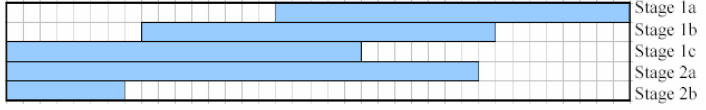
\includegraphics[width=0.85\textwidth,height=0.2\textheight,keepaspectratio]{paper_wastedarea.png}}\\
\subfloat[Modified Wallace Tree from~\cite{betterwallace}. The image reflects the better area utilization based on the algorithm present in the paper.]{\label{fig:paper_improvedarea}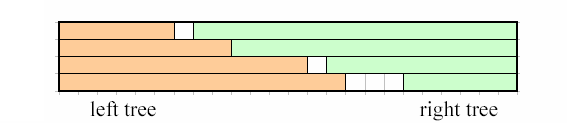
\includegraphics[width=0.85\textwidth,height=0.2\textheight,keepaspectratio]{paper_improvedarea.png}}
\caption{Wallace tree structure before and after the reorganization.}
\label{fig:paper}
\end{figure}


\subsubsection{Implementation and Verification}
\label{sec:implementation}

%IMPLEMENTATION
This section will be used to introduce the reader to the implementation requirements for the multiplier. Followed by a simple, high-level description of the architecture and respective components used to accomplish them. The important handshaking signals will also be explained. It will also feature the procedures used to verify the implementation and what results are expected. Finally the conclusion will close the section.

The implementation tries to closely mimic the three algorithm steps. However additional signals are necessary for the correct interface with the processor. According to the documentation~\cite{doc}~and~\cite{doc2}, there are 3 input signals, \RST, \CLK and \MULI and 1 output signal \MULO. Moreover, there are 4 generics: \infer, \multype, \pipe and \mac. \MULI includes the 32 bit operands (along with an extra signal bit), and several flag to request flushing of the current operation, indicate signed multiplication, to initiate, and to start multiply and accumulate. On the other hand \MULO includes a self explanatory \ready signal, a \nready signal, condition codes that reflect if the result is zero or negative and finally the 64 bit result.

The most significant generic is multype that configures the multiplier to different operand's sizes. These are 16x16, 32x8, 32x16 and 32x32. It is important to note that a discrepancy between the documentation and the actual code exists regarding the multiplier. The infer generic has been replace by tech (related to the target architecture) in the original VHDL file: \texttt{mul32.vhd}. Our custom multiplier replicates this configuration.

The aforementioned ports and generics are summarized in figure~\ref{fig:mul32_dia}.

\begin{figure}[H]
\centering
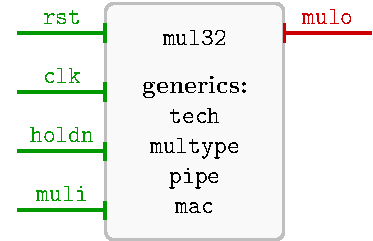
\includegraphics[width=0.70\textwidth,height=0.25\textheight,keepaspectratio]{mul32_dia}
\caption{Diagram of the \texttt{mul32} unit, including all \texttt{in} and \texttt{out} ports as well as generics.}
\label{fig:mul32_dia}
\end{figure}

As mentioned in~\ref{sec:wallace} the algorithm can be divided in three major parts. However to incorporate the starting signal a ``step 0'' was added.

Step 0 is a process that simply monitors the reset and start signals to update some internals signals accordingly. This is important to ensure the multiplier respects the handshaking signals and handles correctly the processor's requests.

On part 1 the operands are \texttt{AND}ed together and their weights are adjusted. To reflect this a three dimensional \STDV was created and named \texttt{WallaceTree}. The first dimension reflects the number of stages (or levels) necessary to finish the operation. These values are computed offline for the four multype possibilities. The second dimension relates to the number of `lines' of the matrix, or its height. The range is always equal to the width of the first operand. Finally, the third dimension accounts for the number of columns, or its width, which is necessarily equal to the sum of the width's of each operand. Figure~\ref{fig:wallace_tree_array} summarizes this information. In practice the 3D array was converted to 1D as synthesis tools have better support for the latter, nonetheless the same principles stand. This step is accomplished in VHDL with \texttt{FOR-GENERATES} and \texttt{IF-GENERATES}. Originally we described this structure with processes, which allowed a more concise and simpler code. However the synthesis tool was not able to complete the synthesization process with the size of the loops we required.

\begin{figure}[H]
\centering
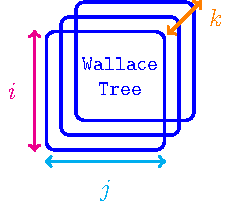
\includegraphics[width=0.6\textwidth,height=0.25\textheight,keepaspectratio]{wallace_tree_array}
\caption{Diagram explaining the structure of the \texttt{WallaceTree} 3D array, with each dimension explicitly shown.}
\label{fig:wallace_tree_array}
\end{figure}

The tree is reorganized so all columns start from the `top', as shown in~\ref{fig:wt_after}. This modification simplifies the implementation of the algorithm for the next steps.

\begin{figure}[H]
\centering
\subfloat[Original]{\label{fig:wt_before}
\includegraphics[width=0.3\textwidth,height=0.2\textheight,keepaspectratio]{wt_before}}\qquad
\subfloat[Modified]{\label{fig:wt_after}
\includegraphics[width=0.3\textwidth,height=0.2\textheight,keepaspectratio]{wt_after}}
\caption{Reorganization of the Wallace tree for easier manipulation in further steps.}
\label{fig:wt_reorganization}
\end{figure}

To be able to multiply signed operands the modified Baugh-Wooley multiplication was used (\emph{cf.}~\cite{part3} and example~\ref{ex:bw}). Therefore some values are complemented if the input is signed. Moreover on the final step a constant value is added to the two operands.
This action completes the first step.

\begin{figure}[H]
\centering
\subfloat[Full Adder]{\label{fig:fa_dia} \begin{minipage}[c][0.20\textheight]{0.45\textwidth} \centering 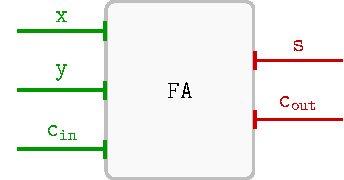
\includegraphics[width=1\textwidth]{fa_dia} \end{minipage}}
\subfloat[Half Adder]{\label{fig:ha_dia} \begin{minipage}[c][0.20\textheight]{0.45\textwidth} \centering 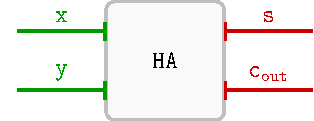
\includegraphics[width=1\textwidth]{ha_dia} \end{minipage}}
\caption{Diagrams describing the interface ports of the Adders used.}
\label{fig:adders_dia}
\end{figure}




Thereafter each group of 3 or 2 bits must be compressed to 1, using full-adders and half-adders respectively (\emph{cf.}~\ref{fig:adders_dia}). If an odd number of bits exist in a certain column the last bit is transferred to the next level. Figure~\ref{fig:wt_compression} assists the reader in understanding the various compressions used. Repeating this process sufficient times\footnote{The exact number of iterations required can be inferred from the integer constant \texttt{levels} previously mentioned.}, the height of the matrix is reduced to 2. These can be added with a conventional adder to determine the final result.

\begin{figure}[H]
\centering
\subfloat[Column with 3 bits.]{\label{fig:wt_3b} \begin{minipage}[c][0.35\textheight]{0.3\textwidth} \centering 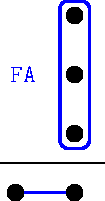
\includegraphics[width=1\textwidth,height=0.35\textheight,keepaspectratio]{wt_3b} \end{minipage}}
\subfloat[Column with 4 bits.]{\label{fig:wt_4b} \begin{minipage}[c][0.35\textheight]{0.35\textwidth} \centering 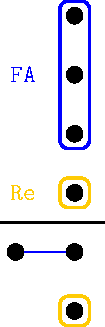
\includegraphics[width=1\textwidth,height=0.35\textheight,keepaspectratio]{wt_4b} \end{minipage}}
\subfloat[Column with 5 bits.]{\label{fig:wt_5b} \begin{minipage}[c][0.35\textheight]{0.35\textwidth} \centering 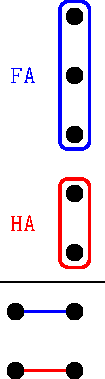
\includegraphics[width=1\textwidth,height=0.35\textheight,keepaspectratio]{wt_5b} \end{minipage}}
\caption{Compressing columns in the WallaceTree with Full Adders and Half Adders. Each example features on column of the tree in level $k$ (before compression) and $k+1$ (after compression).}
\label{fig:wt_compression}
\end{figure}


To help with these operations the exact number of full-adders and half-adders for each column of each stage were precomputed\footnote{The precomputation was performed with a C program which simply runs the algorithm sequentially to determine the necessary components on each column for all stages.}. Moreover two other constants arrays exist that indicate the number of carry ins each column receives and if it has a remainder bit (odd numbered of lines).
Having this information the location of the appropriate inputs (x, y and carry in for the full adder) and outputs (s and carry out) are mapped to a full (or half) adder instance to determine the result.

Step 3 is a process responsible to add with the first two `lines' of the last stage of the \texttt{WallaceTree} signal which yields the final result. However, if the multiplication is signed an extra \STDV is added to these, as explained in~\cite{part3}. Moreover the condition codes are also computed.

%VERIFICATION

In order to verify the correct behaviour of the modified multiplier it was fundamental to write a simple but comprehensive testbench.
Other than all the aforementioned input and output signals the testbench also features some debugging signals that were used during the development phase to observe the behavior of (otherwise) internal signals. The debugging signals were compared to the output of a C program that replicated the desired behavior for the multiplier. This way it was possible to look for differences in the VHDL signals and C \texttt{printf}'s to easily spot bugs as close as possible to their origin. The advantages of using this method cannot be understated as it allowed us to efficiently debug the VHDL code, notably step 2 of the algorithm.

To test our design several combinations of \holdn and \start signals were used in out testbench. In particular changing their frequency with respect to the frequency of the operands.
Regarding the latter, the design was tested with operands close to the maximum allowed (\eg for 32x32, $2^{32} \times 2^{32}-1$, or $\unaryminus 2^{32} \times \unaryminus 2^{32}-1$) and also around 0. Also multiplying two negative values, or one positive and one negative.

An example describing the evolution of the signals driven by our testbench is shown in~\ref{fig:mul32_wave}.

\begin{figure}[H]
\centering
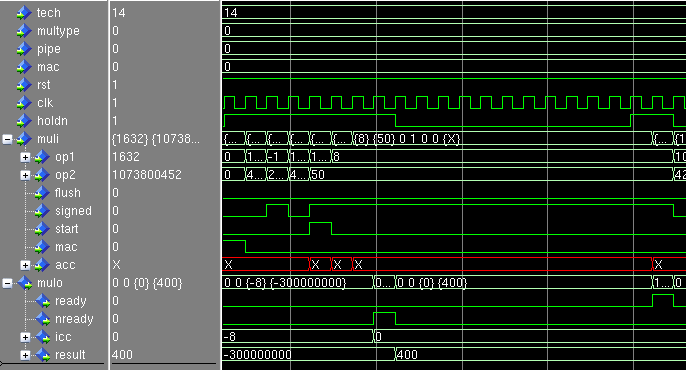
\includegraphics[width=1\textwidth,height=0.4\textheight,keepaspectratio]{handshaking_modified_noholdn.png}
\caption{Screenshot of the Modelsim's Wave for the multiplier. For this particular simulation a 16x16 operation is shown, along with all the appropriate signals.}
\label{fig:mul32_wave}
\end{figure}

The last phase of the verification procedure was to run the Dhrystone testbench in Multisim to determine if the variables match the expected values. When this did not occur we compared the wave results (only the signals relevant to multiplication) of our design with the original's to look for discrepancies. This way it was possible to observe the correct behavior of the handshaking signals, markedly \start, \holdn, \ready and \nready. This type of ``reverse engineering'' was needed as the information in documentation does not concur with the implementation. In addition their behavior changes for different multiplier latency configurations (chosen through \texttt{make xconfig}). For the final design we selected 4-cycles of latency\footnote{It was necessary to perform this change otherwise the processor would not be able to handle the shorter latency of the modified multiplier.} consequently we will only focus on the handshaking signals for this setup. Figure~\ref{fig:handshake} features two wave signals from Modelsim.

\begin{figure}[H]
\centering
\subfloat[With constant \holdn]{\label{fig:mul32_noholdn}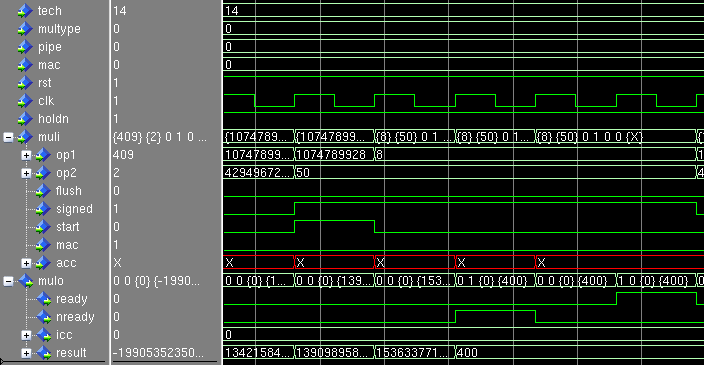
\includegraphics[width=1\textwidth,height=0.5\textheight,keepaspectratio]{handshaking_original_noholdn}}\\
\subfloat[With varying \holdn]{\label{fig:mul32_holdn}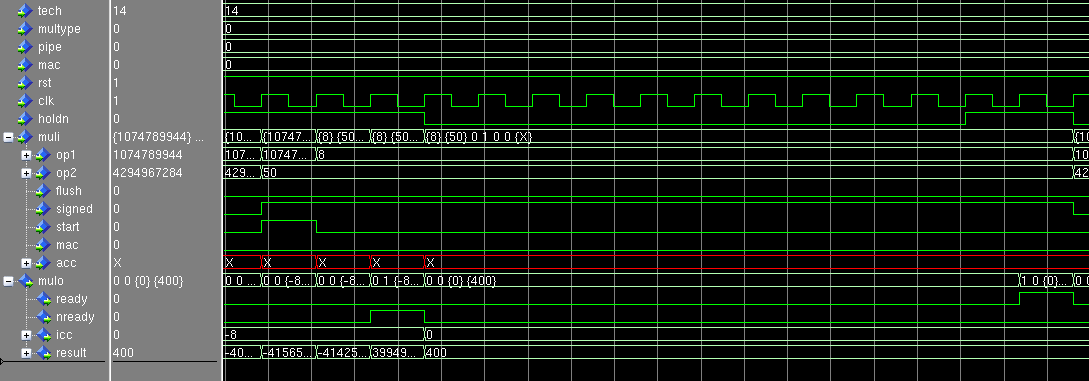
\includegraphics[width=1\textwidth,height=0.5\textheight,keepaspectratio]{handshaking_original_holdn}}\quad
\caption{Detail of the handshaking signals in the original multiplier for the Dhrystone benchmark.}
\label{fig:handshake}
\end{figure}

Relying on the simulations we were able to determine that the operands are read at the falling edge of the muli.start signal. Also the ready signal is raised three cycles after that moment (assuming holdn does not change). The nready signal is set two clock cycle prior to ready.
This information is summarized in the multiplier's state machine depicted in figure~\ref{fig:mul32_state_machine}.

\begin{figure}[H]
\centering
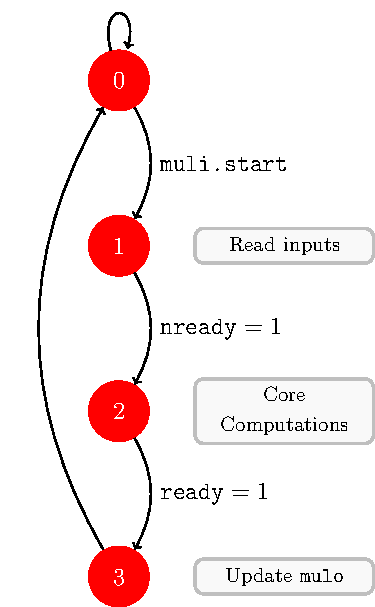
\includegraphics[width=1\textwidth,height=0.5\textheight,keepaspectratio]{mul32_state_machine}
\caption{Diagram explaining how the various handshaking signals behave.}
\label{fig:mul32_state_machine}
\end{figure}


% Conclusion

With this implementation we expect the benchmark results to improvement as the latency of the multiplier was reduced from 5 to 2 cycles. On the other hand, the area and power consumption will likely increase as the Wallace tree makes use of more resources. Some improvements related to better utilization of area are left for future work. In addition other modifications of this design which can have positive impact on metrics would have been interesting to implement and test. Examples include using a Dadda Multiplier (which uses less gates) instead of Wallace's, or using Booth recoding to decrease the size of the operands.


